\documentclass[12pt,a4paper]{report}

%% ─── PACKAGES ────────────────────────────────────────────────────────────────
\usepackage[utf8]{inputenc}
\usepackage[T1]{fontenc}
\usepackage[margin=1in]{geometry}
\usepackage{graphicx}
\usepackage{fancyhdr}
\usepackage{hyperref}
\usepackage{titlesec}
\usepackage{tocloft}
\usepackage{booktabs}
\usepackage{longtable}
\usepackage{array}
\usepackage{enumitem}
\usepackage{xcolor}
\usepackage{listings}
\usepackage{float}
\usepackage{amsmath}
\usepackage{setspace}
\usepackage{caption}
\usepackage{subcaption}
\usepackage{fontawesome5}
\usepackage{tikz}
\usetikzlibrary{shapes.geometric, arrows.meta, positioning, fit, backgrounds, calc}
\usepackage{pgfplots}
\pgfplotsset{compat=1.18}
\usepackage{multirow}
\usepackage[normalem]{ulem}
\usepackage{mdframed}
\usepackage{parskip}
\usepackage{microtype}
\usepackage{lmodern}

%% ─── COLOR PALETTE ───────────────────────────────────────────────────────────
\definecolor{GreenPrimary}{HTML}{2E7D32}
\definecolor{GreenLight}{HTML}{4CAF50}
\definecolor{GreenDark}{HTML}{1B5E20}
\definecolor{AccentGold}{HTML}{F9A825}
\definecolor{TextMuted}{HTML}{555555}
\definecolor{LightBg}{HTML}{F1F8E9}
\definecolor{CodeBg}{HTML}{F5F5F5}
\definecolor{DFDProcess}{HTML}{A5D6A7}
\definecolor{DFDExternal}{HTML}{90CAF9}
\definecolor{DFDStore}{HTML}{FFE082}
\definecolor{DFDFlow}{HTML}{546E7A}

%% ─── HYPERREF ────────────────────────────────────────────────────────────────
\hypersetup{
  colorlinks=true,
  linkcolor=GreenDark,
  urlcolor=GreenPrimary,
  citecolor=GreenDark,
  pdftitle={GreenNest Indoor Plant E-Commerce Platform},
  pdfauthor={Pawan Pokharel},
}

%% ─── HEADER/FOOTER ───────────────────────────────────────────────────────────
\pagestyle{fancy}
\fancyhf{}
\fancyhead[L]{\small\textcolor{GreenPrimary}{\textbf{GreenNest}}}
\fancyhead[R]{\small\textcolor{TextMuted}{\leftmark}}
\fancyfoot[C]{\thepage}
\renewcommand{\headrulewidth}{0.4pt}
\renewcommand{\headrule}{\hbox to\headwidth{\color{GreenPrimary}\leaders\hrule height \headrulewidth\hfill}}

%% ─── CHAPTER TITLE FORMAT ────────────────────────────────────────────────────
\titleformat{\chapter}[display]
  {\normalfont\huge\bfseries\color{GreenDark}}
  {\chaptertitlename\ \thechapter}{20pt}{\Huge}
\titlespacing*{\chapter}{0pt}{-20pt}{40pt}

\titleformat{\section}{\large\bfseries\color{GreenPrimary}}{{\thesection}}{1em}{}
\titleformat{\subsection}{\normalsize\bfseries\color{GreenDark}}{{\thesubsection}}{1em}{}

%% ─── CODE LISTINGS ───────────────────────────────────────────────────────────
\lstset{
  backgroundcolor=\color{CodeBg},
  basicstyle=\ttfamily\small,
  breaklines=true,
  frame=single,
  rulecolor=\color{GreenLight},
  keywordstyle=\color{GreenDark}\bfseries,
  commentstyle=\color{TextMuted}\itshape,
  stringstyle=\color{AccentGold},
  numbers=left,
  numberstyle=\tiny\color{TextMuted},
  showstringspaces=false,
  tabsize=4,
}

%% ─── TIKZ STYLES FOR DFD ─────────────────────────────────────────────────────
\tikzset{
  external/.style={
    rectangle, draw=GreenDark, thick,
    fill=DFDExternal, text centered,
    minimum width=2.5cm, minimum height=1cm,
    font=\small\bfseries, rounded corners=2pt
  },
  process/.style={
    ellipse, draw=GreenPrimary, thick,
    fill=DFDProcess, text centered,
    minimum width=3cm, minimum height=1.2cm,
    font=\small\bfseries
  },
  datastore/.style={
    rectangle, draw=GreenPrimary, thick,
    fill=DFDStore, text centered,
    minimum width=3cm, minimum height=0.8cm,
    font=\small, path picture={
      \draw[thick] (path picture bounding box.north west) -- (path picture bounding box.north east);
      \draw[thick] (path picture bounding box.south west) -- (path picture bounding box.south east);
    }
  },
  flow/.style={
    ->, thick, color=DFDFlow, >=Stealth
  },
}

%% ─── BEGIN DOCUMENT ──────────────────────────────────────────────────────────
\begin{document}

%% ──────────────────────────────────────────────────────────────────────────────
%%  TITLE PAGE
%% ──────────────────────────────────────────────────────────────────────────────
\begin{titlepage}
  \centering

  {\large \textbf{Tribhuvan University}\\
  Institute of Science and Technology}\\[0.5em]
  {\normalsize Bachelor of Science in Computer Science and Information Technology}\\[2em]

  \textcolor{GreenPrimary}{\rule{\linewidth}{2pt}}\\[1em]

  {\Huge\bfseries\color{GreenDark} GreenNest}\\[0.5em]
  {\LARGE\color{GreenPrimary} Indoor Plant E-Commerce Platform}\\[1em]
  {\large\color{TextMuted} A Web-Based B2C Plant Retail System for the Kathmandu Valley}\\[1em]

  \textcolor{GreenPrimary}{\rule{\linewidth}{1pt}}\\[1.5em]

  \includegraphics[width=8cm]{public/favicon.ico}

  \vspace{1.5em}

  \begin{tabular}{rl}
    \textbf{Submitted By:}   & Pawan Pokharel \\
    \textbf{Roll No.:}       & TU/2024/BSCCSIT/XXX \\
    \textbf{Submitted To:}   & Department of Computer Science and IT \\
    \textbf{Submission Date:}& \today \\
  \end{tabular}

  \vfill

  {\small\color{TextMuted}
    GreenNest Indoor Plants \quad | \quad Kathmandu, Nepal\\
    \url{https://greennest.com.np}
  }
\end{titlepage}

%% ──────────────────────────────────────────────────────────────────────────────
%%  ABSTRACT
%% ──────────────────────────────────────────────────────────────────────────────
\thispagestyle{plain}
\begin{center}
  {\LARGE\bfseries\color{GreenDark} Abstract}
\end{center}
\vspace{1em}

\onehalfspacing

GreenNest is a full-stack, production-ready B2C (Business-to-Consumer) indoor plant e-commerce platform developed specifically for the Nepalese market. The system enables residents of the Kathmandu Valley and broader urban centres of Nepal to browse, discover, and purchase high-quality indoor plants online, with delivery to their doorstep.

The platform integrates Nepal's dominant digital payment gateway, \textbf{eSewa ePay v2}, providing a secure and familiar checkout experience for Nepalese customers alongside the traditional Cash on Delivery (COD) method. Payment verification is implemented using HMAC-SHA256 server-side signature validation to ensure transaction integrity.

The application is built on \textbf{Laravel 13} (PHP 8.3), \textbf{MySQL 8.0}, and styled with \textbf{Tailwind CSS}, offering a mobile-first, responsive user interface. A comprehensive admin panel facilitates product catalogue management, order lifecycle tracking, customer administration, and real-time inventory control.

This report documents the complete software development lifecycle of GreenNest: background study, system analysis, feasibility study, requirements specification, architectural design, data flow diagrams, database design, implementation, testing, and conclusions.

\newpage

%% ──────────────────────────────────────────────────────────────────────────────
%%  TABLE OF CONTENTS
%% ──────────────────────────────────────────────────────────────────────────────
\tableofcontents
\newpage
\listoffigures
\newpage
\listoftables
\newpage

%% ══════════════════════════════════════════════════════════════════════════════
\chapter{Introduction}
%% ══════════════════════════════════════════════════════════════════════════════

\section{Background}

Nepal is undergoing a rapid urban transition. According to the Central Bureau of Statistics (CBS Nepal, 2021), the urban population has grown to approximately \textbf{21\%} of the total population, with the Kathmandu Valley alone housing over 2.5 million residents. Rising disposable incomes, apartment-style living, and increased environmental consciousness have sparked a significant interest in indoor plants and urban greenery.

Indoor plants are no longer a luxury—they have become an essential element of modern Nepalese interior design. Trends driven by social media platforms—particularly Instagram and Facebook, which collectively boast over \textbf{15 million Nepalese users}—have accelerated consumer interest in aesthetically appealing and air-purifying indoor plants.

Despite this growing demand, the indoor plant retail sector in Nepal remains largely unorganised. Most plant purchases occur at physical nurseries concentrated in areas such as \textbf{Thapathali, Balkhu, and Imadol} in Kathmandu, \textbf{Pulchowk} in Lalitpur, and \textbf{Banepa} in Kavrepalanchok. These markets suffer from:

\begin{itemize}
  \item \textbf{Geographic inaccessibility} — customers must travel significant distances.
  \item \textbf{Limited product information} — no care instructions, difficulty information, or watering schedules.
  \item \textbf{Cash-only transactions} — no digital payment integration.
  \item \textbf{No home delivery} — particularly problematic during monsoon and extreme weather.
  \item \textbf{Seasonal availability uncertainty} — no inventory visibility.
\end{itemize}

\textbf{GreenNest} addresses all these pain-points by providing a curated, digital marketplace for indoor plants in Nepal.

\section{Problem Statement}

Despite Nepal's growing urban population and rising demand for indoor plants, there exists no dedicated, professionally structured e-commerce platform in Nepal catering exclusively to indoor plant retail. Existing generic e-commerce platforms (Daraz, HamroBazar) either lack plant-specific features such as care guides, light/water requirements, and difficulty ratings, or fail to provide a curated, trusted plant-buying experience.

Furthermore, the absence of a Nepal-native payment gateway integration (eSewa) in plant-specific platforms means customers are forced to rely solely on cash transactions, creating friction and discouraging impulse purchases.

\section{Objectives}

The primary objectives of the GreenNest platform are:

\begin{enumerate}
  \item Develop a full-featured, mobile-responsive e-commerce platform specifically for indoor plant retail in Nepal.
  \item Integrate \textbf{eSewa ePay v2} as the primary digital payment gateway with server-side HMAC-SHA256 signature verification.
  \item Provide plant-specific product metadata (light requirements, watering schedules, difficulty ratings) to empower informed purchasing decisions.
  \item Implement a comprehensive \textbf{Admin Panel} with real-time inventory, order lifecycle management, and customer administration.
  \item Enable search, filtering, and sorting by category, price, and care difficulty to aid product discovery.
  \item Facilitate delivery to the \textbf{Kathmandu Valley} (Kathmandu, Lalitpur, Bhaktapur districts).
\end{enumerate}

\section{Scope}

\subsection{Included in Scope}
\begin{itemize}
  \item Customer-facing storefront: product catalogue, search, category filters, product detail pages.
  \item Shopping cart with session/database persistence.
  \item User authentication (registration, login, password management).
  \item Checkout with \textbf{eSewa ePay v2} and \textbf{Cash on Delivery}.
  \item Order management: placement, confirmation, tracking, cancellation.
  \item Admin panel: product/category CRUD, order management, user management, settings.
  \item Deployment target: \textbf{cPanel shared hosting} with PHP 8.3.
\end{itemize}

\subsection{Excluded from Scope}
\begin{itemize}
  \item Mobile application (iOS/Android).
  \item Multi-vendor marketplace.
  \item Logistics/courier integration API.
  \item International shipping.
  \item Social media login (OAuth).
\end{itemize}

\section{Report Organisation}

The remainder of this report is structured as follows: Chapter 2 covers the background study and literature review. Chapter 3 presents system analysis including the feasibility study. Chapter 4 describes the system design with data flow diagrams and database schema. Chapter 5 covers the implementation. Chapter 6 details testing and validation. Chapter 7 provides conclusions and future work.

%% ══════════════════════════════════════════════════════════════════════════════
\chapter{Background Study}
%% ══════════════════════════════════════════════════════════════════════════════

\section{Nepal's Digital Economy Context}

Nepal's digital economy has grown substantially post-2020. Key indicators include:

\begin{table}[H]
\centering
\caption{Nepal Digital Economy Indicators (2024)}
\begin{tabular}{@{}lll@{}}
\toprule
\textbf{Indicator} & \textbf{Value} & \textbf{Source} \\
\midrule
Internet Penetration         & 76.4\%             & NTA, 2024 \\
Mobile Internet Users        & 24.8 million       & NTA, 2024 \\
eSewa Registered Users       & 8+ million         & eSewa, 2024 \\
Khalti Users                 & 4+ million         & Khalti, 2024 \\
E-commerce Market Size (NPR) & Rs. 15+ billion    & DoCS, 2023 \\
Smartphone Penetration       & 62\%               & GSMA, 2023 \\
\bottomrule
\end{tabular}
\end{table}

\section{eSewa Payment Gateway}

eSewa, operated by F1Soft International Pvt. Ltd. (a subsidiary of CG Digital), is Nepal's first and largest digital wallet. With over 8 million registered users and acceptance at 50,000+ merchants, it is the dominant digital payment method in Nepal.

eSewa ePay v2 provides:
\begin{itemize}
  \item HMAC-SHA256 transaction signature verification.
  \item Real-time payment notification via callback URL.
  \item Test and live environments (RC and production).
  \item Web and mobile redirect-based payment flow.
\end{itemize}

GreenNest implements eSewa ePay v2 with \textbf{server-side signature generation} (never exposing the secret key to the client) and \textbf{server-side callback verification} before marking an order as paid.

\section{Existing Platforms in Nepal}

\begin{table}[H]
\centering
\caption{Comparative Analysis of Relevant Nepalese Platforms}
\begin{tabular}{@{}lccccl@{}}
\toprule
\textbf{Platform} & \textbf{Plant-specific} & \textbf{eSewa} & \textbf{Care Info} & \textbf{Admin Panel} & \textbf{Focus} \\
\midrule
Daraz Nepal       & \texttimes & \checkmark & \texttimes & \texttimes & General e-commerce \\
HamroBazar        & \texttimes & \checkmark & \texttimes & \texttimes & Classifieds \\
SastoDeal         & \texttimes & \checkmark & \texttimes & Limited     & Electronics/grocery\\
Local nurseries   & \checkmark & \texttimes & \texttimes & \texttimes & Physical retail \\
\textbf{GreenNest}& \textbf{\checkmark} & \textbf{\checkmark} & \textbf{\checkmark} & \textbf{\checkmark} & \textbf{Indoor plants} \\
\bottomrule
\end{tabular}
\end{table}

\section{Technology Stack Rationale}

\begin{description}
  \item[\textbf{Laravel 13}] — PHP's most mature MVC framework with built-in features for authentication, routing, ORM (Eloquent), payments, and security.
  \item[\textbf{MySQL 8.0}] — Industry-standard RDBMS, widely supported on Nepalese shared hosting providers such as Hostinger Nepal and WebsiteNepal.
  \item[\textbf{Tailwind CSS}] — Utility-first CSS framework enabling rapid, consistent UI development.
  \item[\textbf{Vite}] — Next-generation frontend bundler for fast HMR during development.
\end{description}

%% ══════════════════════════════════════════════════════════════════════════════
\chapter{System Analysis}
%% ══════════════════════════════════════════════════════════════════════════════

\section{Feasibility Study}

\subsection{Technical Feasibility}
The system is built on mature, well-documented technologies (Laravel, MySQL, PHP 8.3). All components are open-source and freely available. Deployment requires standard cPanel shared hosting (available in Nepal from Rs. 2,000/year), making it technically and economically accessible.

\subsection{Operational Feasibility}
\begin{itemize}
  \item \textbf{Customer side}: Customers with a smartphone and internet connection can place orders. The mobile-first UI supports low-bandwidth connections.
  \item \textbf{Admin side}: The admin panel requires only a web browser, usable on any device.
  \item \textbf{Payment}: eSewa accounts are free to open, with a user base exceeding 8 million in Nepal.
\end{itemize}

\subsection{Economic Feasibility}
\begin{table}[H]
\centering
\caption{Estimated Development and Operational Costs (NPR)}
\begin{tabular}{@{}lrr@{}}
\toprule
\textbf{Item} & \textbf{One-time (NPR)} & \textbf{Annual (NPR)} \\
\midrule
Domain (.com.np)          & 1,500  & 1,500  \\
Shared Hosting (cPanel)   & —      & 5,500  \\
SSL Certificate           & —      & Free (Let's Encrypt) \\
eSewa Merchant Activation & 5,000  & — \\
Development (in-house)    & 0      & — \\
\midrule
\textbf{Total}            & \textbf{6,500} & \textbf{7,000} \\
\bottomrule
\end{tabular}
\end{table}

\subsection{Schedule Feasibility}
The platform was developed in approximately 6 weeks, well within a typical university semester project timeline.

\section{Requirements Specification}

\subsection{Functional Requirements}

\begin{longtable}{@{}lp{10cm}@{}}
\caption{Functional Requirements} \\
\toprule
\textbf{ID} & \textbf{Requirement} \\
\midrule
\endfirsthead
\multicolumn{2}{c}{\tablename\ \thetable\ — Continued} \\
\toprule
\textbf{ID} & \textbf{Requirement} \\
\midrule
\endhead
FR-01 & Customer shall be able to register with name, email, phone, and address. \\
FR-02 & Customer shall be able to log in with email and password. \\
FR-03 & Customer shall be able to browse products by category. \\
FR-04 & Customer shall be able to search products by keyword. \\
FR-05 & Customer shall be able to filter products by price, light, and difficulty. \\
FR-06 & Customer shall be able to view full product details including care information. \\
FR-07 & Customer shall be able to add/remove items from the shopping cart. \\
FR-08 & Customer shall be able to update item quantities in the cart. \\
FR-09 & Customer shall be able to checkout using eSewa digital payment. \\
FR-10 & Customer shall be able to checkout using Cash on Delivery. \\
FR-11 & System shall verify eSewa payments via HMAC-SHA256 before confirming order. \\
FR-12 & Customer shall receive an order confirmation page after successful checkout. \\
FR-13 & Customer shall be able to view order history and current order status. \\
FR-14 & Customer shall be able to cancel a pending order. \\
FR-15 & Admin shall be able to add, edit, and delete product listings. \\
FR-16 & Admin shall be able to manage product categories with icons. \\
FR-17 & Admin shall be able to view and update order status. \\
FR-18 & Admin shall be able to view and manage customer accounts. \\
FR-19 & Admin shall be able to configure store settings (name, banners, discounts). \\
FR-20 & System shall decrement stock quantity upon order confirmation. \\
\bottomrule
\end{longtable}

\subsection{Non-Functional Requirements}

\begin{table}[H]
\centering
\caption{Non-Functional Requirements}
\begin{tabular}{@{}llp{8cm}@{}}
\toprule
\textbf{ID} & \textbf{Category} & \textbf{Requirement} \\
\midrule
NFR-01 & Performance    & Page load time < 3 seconds on 4G connection. \\
NFR-02 & Security       & All routes protected by CSRF tokens. \\
NFR-03 & Security       & Passwords hashed using bcrypt. \\
NFR-04 & Security       & Payment signatures verified server-side only. \\
NFR-05 & Usability      & Mobile-first, responsive on 320px–1920px viewports. \\
NFR-06 & Availability   & 99.5\% uptime on shared hosting. \\
NFR-07 & Maintainability& Code follows PSR-12 PHP coding standards. \\
NFR-08 & Localisation   & Prices displayed in Nepalese Rupees (NPR, Rs.). \\
\bottomrule
\end{tabular}
\end{table}

%% ══════════════════════════════════════════════════════════════════════════════
\chapter{System Design}
%% ══════════════════════════════════════════════════════════════════════════════

\section{System Architecture}

GreenNest follows the \textbf{Model-View-Controller (MVC)} architectural pattern as enforced by the Laravel framework. The high-level architecture is depicted below.

\begin{figure}[H]
\centering
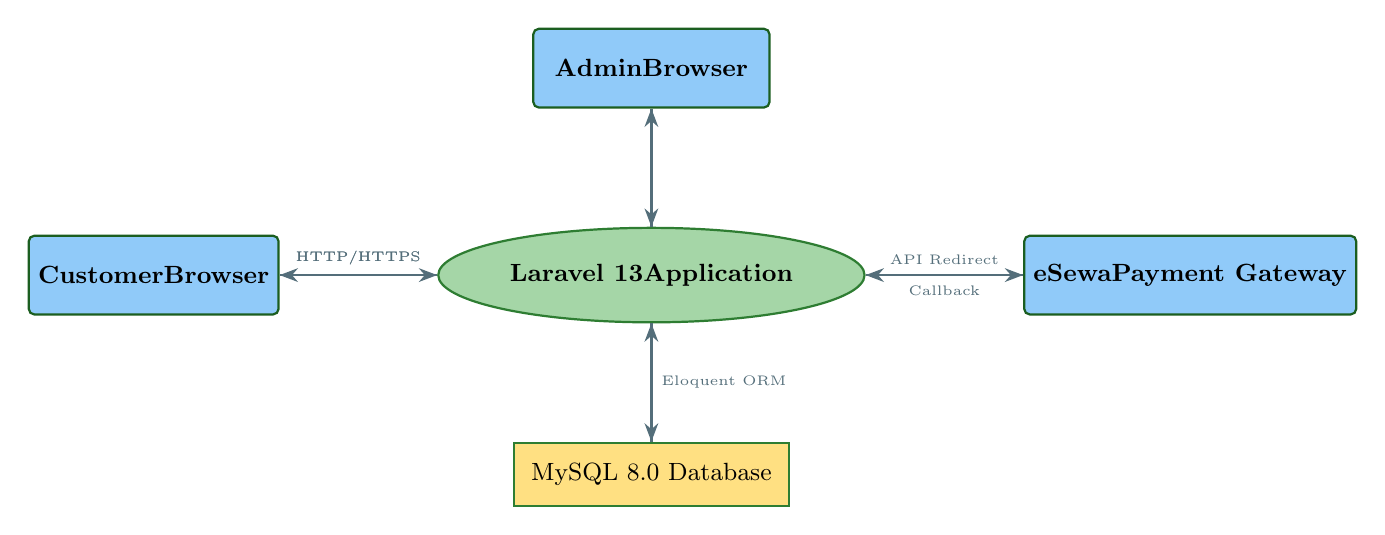
\begin{tikzpicture}[node distance=1.5cm, every node/.style={font=\small}]
  % Browser
  \node[external, minimum width=3cm] (browser) {Customer\\Browser};

  % Laravel App
  \node[process, right=2cm of browser, minimum width=4cm] (app) {Laravel 13\\Application};

  % MySQL
  \node[datastore, below=1.5cm of app, minimum width=3.5cm] (db) {MySQL 8.0 Database};

  % eSewa
  \node[external, right=2cm of app, minimum width=3cm] (esewa) {eSewa\\Payment Gateway};

  % Admin
  \node[external, above=1.5cm of app, minimum width=3cm] (admin) {Admin\\Browser};

  % Arrows
  \draw[flow] (browser) -- node[above, font=\tiny]{HTTP/HTTPS} (app);
  \draw[flow] (app) -- node[above, font=\tiny]{HTTP/HTTPS} (browser);
  \draw[flow] (app) -- node[right, font=\tiny]{Eloquent ORM} (db);
  \draw[flow] (db) -- (app);
  \draw[flow] (app) -- node[above, font=\tiny]{API Redirect} (esewa);
  \draw[flow] (esewa) -- node[below, font=\tiny]{Callback} (app);
  \draw[flow] (admin) -- (app);
  \draw[flow] (app) -- (admin);
\end{tikzpicture}
\caption{High-Level System Architecture}
\end{figure}

\section{Data Flow Diagram — Level 0 (Context Diagram)}

The Level 0 DFD, also known as the \textbf{Context Diagram}, shows GreenNest as a single process interacting with external entities.

\begin{figure}[H]
\centering
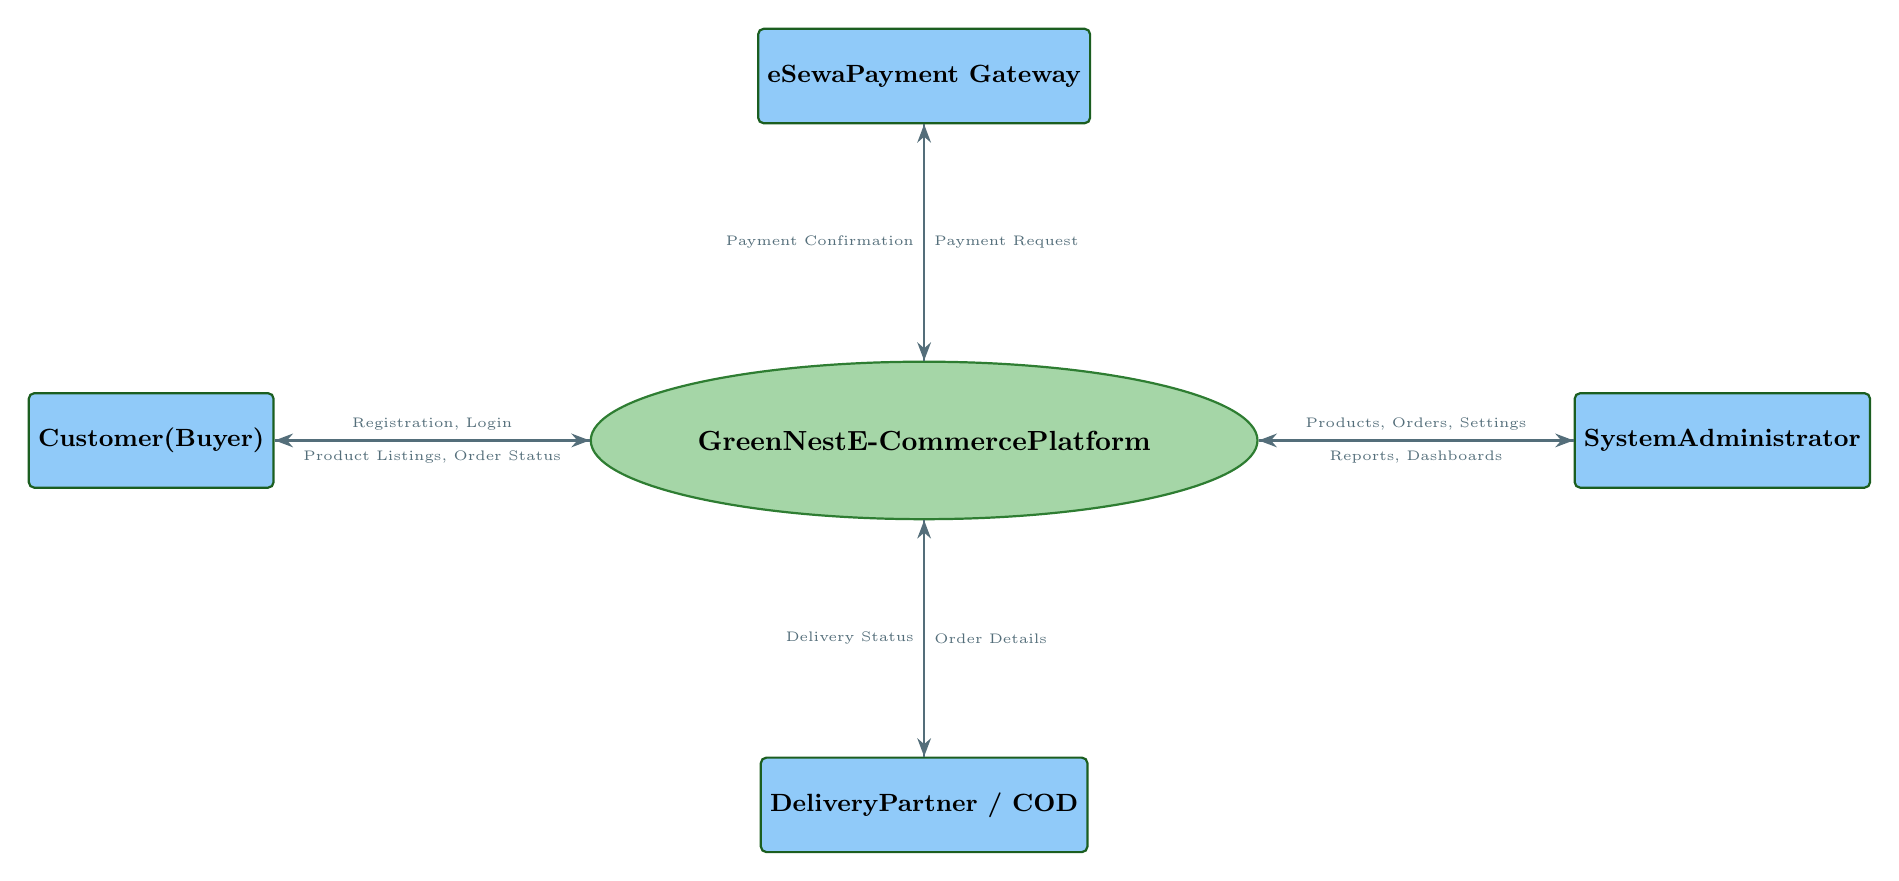
\begin{tikzpicture}[node distance=3cm, every node/.style={font=\small}]

  % Central process
  \node[process, minimum width=5cm, minimum height=2cm, font=\normalsize\bfseries] (system)
    {GreenNest\\E-Commerce\\Platform};

  % External entities
  \node[external, left=4cm of system, minimum height=1.2cm] (customer) {Customer\\(Buyer)};
  \node[external, right=4cm of system, minimum height=1.2cm] (admin) {System\\Administrator};
  \node[external, above=3cm of system, minimum height=1.2cm] (esewa) {eSewa\\Payment Gateway};
  \node[external, below=3cm of system, minimum height=1.2cm] (courier) {Delivery\\Partner / COD};

  % Customer flows
  \draw[flow] (customer) -- node[above, sloped, font=\tiny]{Registration, Login}(system);
  \draw[flow] (system) -- node[below, sloped, font=\tiny]{Product Listings, Order Status}(customer);

  % eSewa flows
  \draw[flow] (system) -- node[right, font=\tiny]{Payment Request}(esewa);
  \draw[flow] (esewa) -- node[left, font=\tiny]{Payment Confirmation}(system);

  % Admin flows
  \draw[flow] (admin) -- node[above, sloped, font=\tiny]{Products, Orders, Settings}(system);
  \draw[flow] (system) -- node[below, sloped, font=\tiny]{Reports, Dashboards}(admin);

  % Courier flows
  \draw[flow] (system) -- node[right, font=\tiny]{Order Details}(courier);
  \draw[flow] (courier) -- node[left, font=\tiny]{Delivery Status}(system);

\end{tikzpicture}
\caption{DFD Level 0 — Context Diagram}
\end{figure}

\section{Data Flow Diagram — Level 1}

The Level 1 DFD decomposes GreenNest into its six major functional processes:

\begin{figure}[H]
\centering
\resizebox{\textwidth}{!}{%
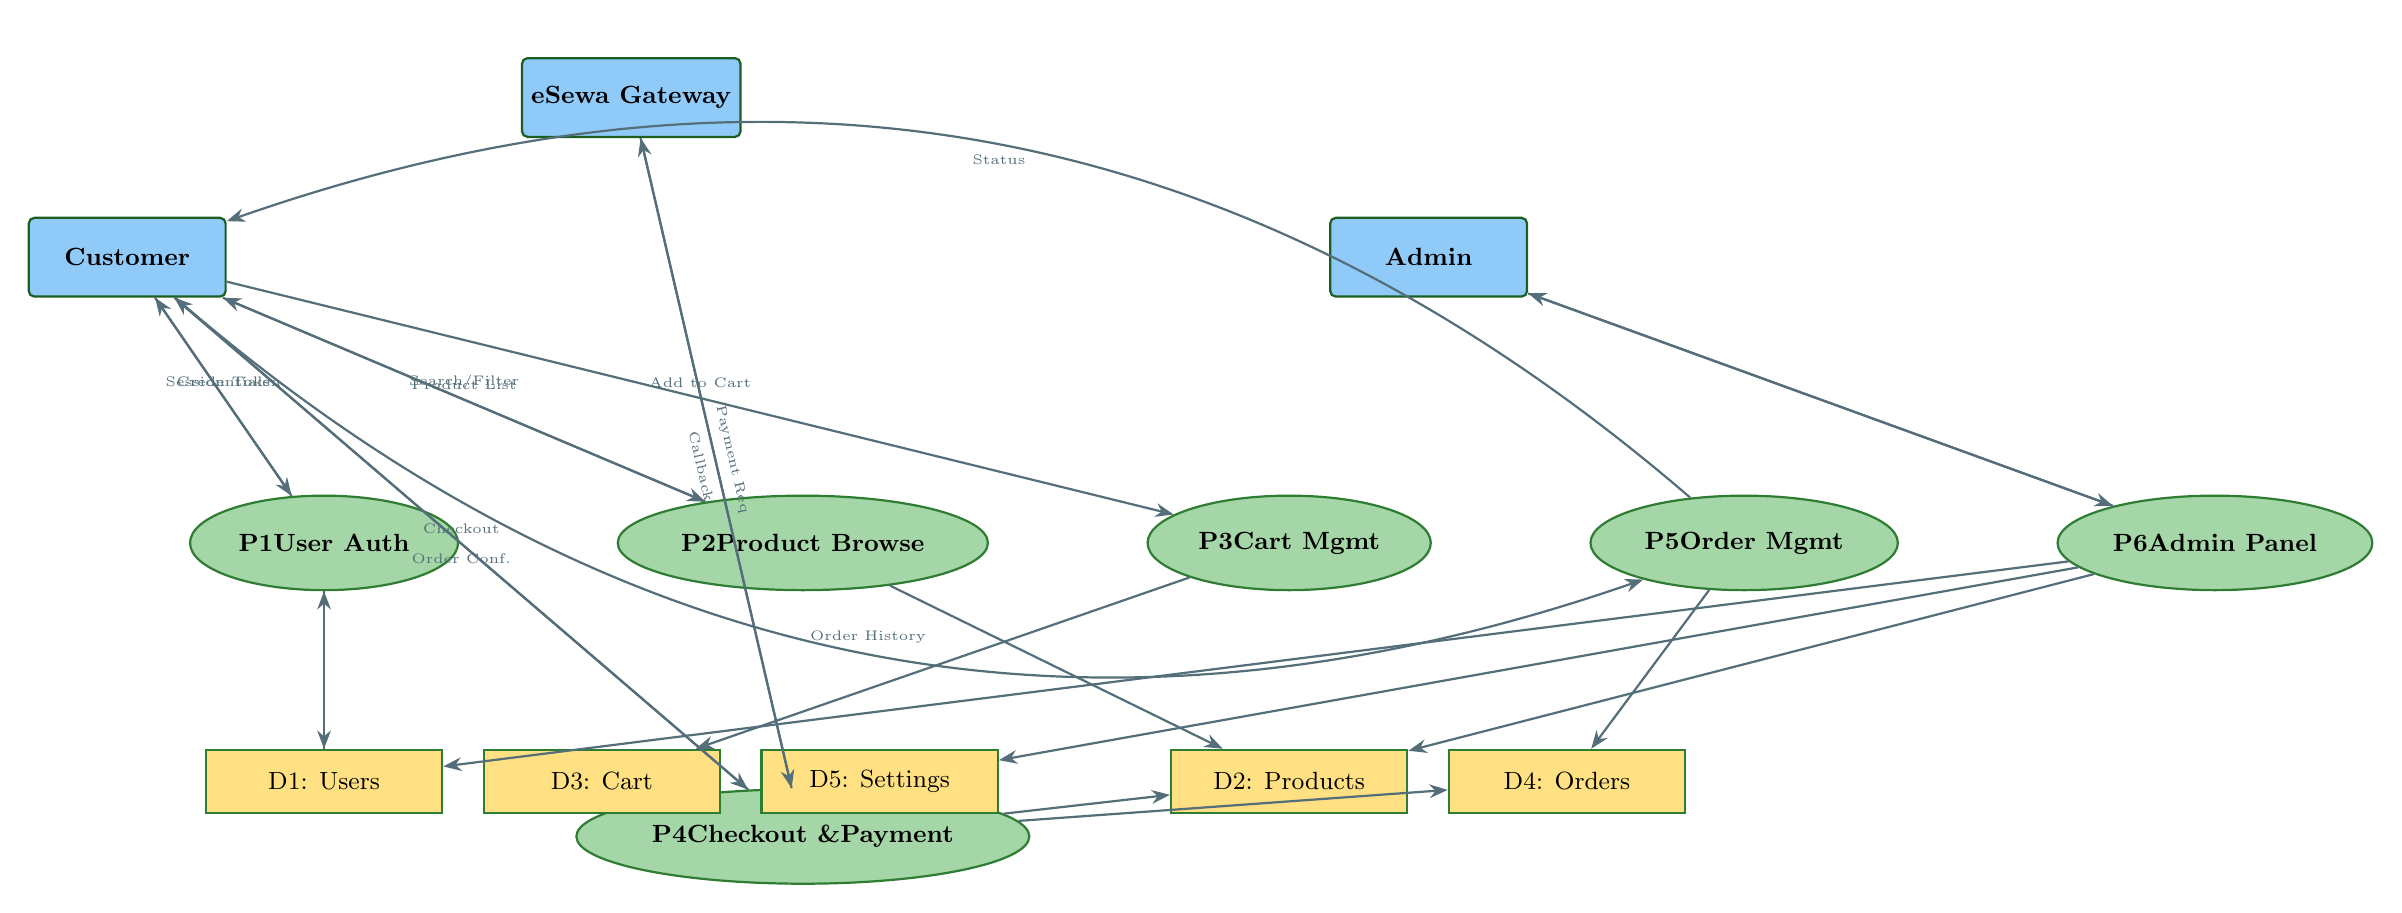
\begin{tikzpicture}[node distance=2cm, every node/.style={font=\scriptsize}]

  %% External entities
  \node[external] (cust) {Customer};
  \node[external, right=14cm of cust] (admin) {Admin};
  \node[external, above=1cm of cust, anchor=south west, xshift=5cm] (esewa) {eSewa Gateway};

  %% Processes
  \node[process, below=2.5cm of cust, xshift=2.5cm]  (p1) {P1\\User Auth};
  \node[process, right=2cm of p1]        (p2) {P2\\Product Browse};
  \node[process, right=2cm of p2]        (p3) {P3\\Cart Mgmt};
  \node[process, below=2.5cm of p2]      (p4) {P4\\Checkout \&\\Payment};
  \node[process, right=2cm of p3]        (p5) {P5\\Order Mgmt};
  \node[process, right=2cm of p5]        (p6) {P6\\Admin Panel};

  %% Data Stores
  \node[datastore, below=2cm of p1]      (ds1) {D1: Users};
  \node[datastore, below=2cm of p3]      (ds2) {D2: Products};
  \node[datastore, right=0.5cm of ds1]   (ds3) {D3: Cart};
  \node[datastore, right=0.5cm of ds2]   (ds4) {D4: Orders};
  \node[datastore, right=0.5cm of ds3]   (ds5) {D5: Settings};

  %% Customer flows
  \draw[flow] (cust) -- node[above]{\tiny Credentials} (p1);
  \draw[flow] (p1)   -- node[above]{\tiny Session Token} (cust);
  \draw[flow] (cust) -- node[above]{\tiny Search/Filter} (p2);
  \draw[flow] (p2)   -- node[above]{\tiny Product List} (cust);
  \draw[flow] (cust) -- node[above]{\tiny Add to Cart} (p3);
  \draw[flow] (cust) -- node[above]{\tiny Checkout} (p4);
  \draw[flow] (p4)   -- node[below]{\tiny Order Conf.} (cust);
  \draw[flow] (cust) to[bend right] node[above]{\tiny Order History} (p5);
  \draw[flow] (p5)   to[bend right] node[below]{\tiny Status} (cust);

  %% eSewa flows
  \draw[flow] (p4) -- node[sloped,above]{\tiny Payment Req} (esewa);
  \draw[flow] (esewa) -- node[sloped,below]{\tiny Callback} (p4);

  %% Admin flows
  \draw[flow] (admin) -- (p6);
  \draw[flow] (p6) -- (admin);

  %% Process–Datastore flows
  \draw[flow] (p1) -- (ds1);
  \draw[flow] (ds1) -- (p1);
  \draw[flow] (p2) -- (ds2);
  \draw[flow] (p3) -- (ds3);
  \draw[flow] (p4) -- (ds4);
  \draw[flow] (p4) -- (ds2);
  \draw[flow] (p5) -- (ds4);
  \draw[flow] (p6) -- (ds2);
  \draw[flow] (p6) -- (ds1);
  \draw[flow] (p6) -- (ds5);

\end{tikzpicture}
} % resizebox
\caption{DFD Level 1 — Main System Processes}
\end{figure}

\section{Data Flow Diagram — Level 2: Checkout Process (P4)}

The Level 2 DFD expands the most critical process, \textit{P4: Checkout \& Payment}, showing the detailed sub-processes involved in order placement and eSewa payment verification.

\begin{figure}[H]
\centering
\resizebox{\textwidth}{!}{%
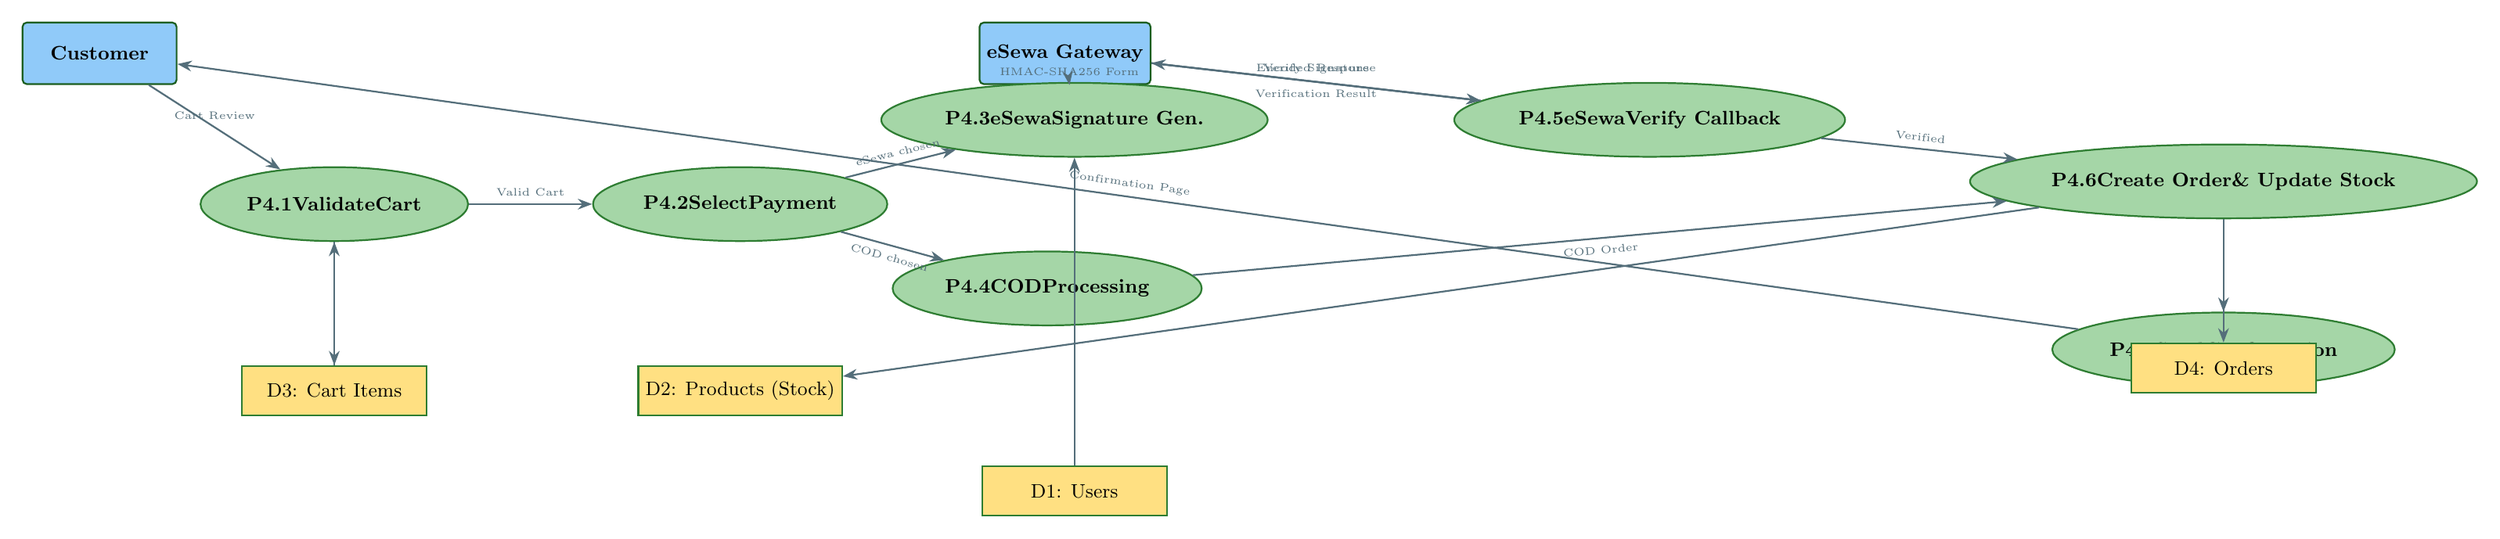
\begin{tikzpicture}[node distance=1.8cm, every node/.style={font=\scriptsize}]

  %% External
  \node[external] (cust) {Customer};
  \node[external, right=13cm of cust] (esewa) {eSewa Gateway};

  %% Processes
  \node[process, below right=1.5cm and 1cm of cust] (p41) {P4.1\\Validate\\Cart};
  \node[process, right=2cm of p41]                   (p42) {P4.2\\Select\\Payment};
  \node[process, above right=0.5cm and 1.5cm of p42] (p43) {P4.3\\eSewa\\Signature Gen.};
  \node[process, below right=0.5cm and 1.5cm of p42] (p44) {P4.4\\COD\\Processing};
  \node[process, right=3cm of p43]                   (p45) {P4.5\\eSewa\\Verify Callback};
  \node[process, right=2cm of p45, yshift=-1cm]      (p46) {P4.6\\Create Order\\\& Update Stock};
  \node[process, below=1.5cm of p46]                 (p47) {P4.7\\Send\\Confirmation};

  %% Data Stores
  \node[datastore, below=2cm of p41]  (ds3) {D3: Cart Items};
  \node[datastore, below=2cm of p46]  (ds4) {D4: Orders};
  \node[datastore, below=2cm of p42]  (ds2) {D2: Products (Stock)};
  \node[datastore, below=5cm of p43]  (ds1) {D1: Users};

  %% Flows
  \draw[flow] (cust) -- node[above]{\tiny Cart Review} (p41);
  \draw[flow] (p41) -- node[above]{\tiny Valid Cart} (p42);
  \draw[flow] (p41) -- (ds3);
  \draw[flow] (ds3) -- (p41);

  \draw[flow] (p42) -- node[sloped,above]{\tiny eSewa chosen} (p43);
  \draw[flow] (p42) -- node[sloped,below]{\tiny COD chosen} (p44);

  \draw[flow] (p43) -- node[above]{\tiny HMAC-SHA256 Form} (esewa);
  \draw[flow] (esewa) -- node[above]{\tiny Encoded Response} (p45);
  \draw[flow] (p45) -- node[above]{\tiny Verify Signature} (esewa);
  \draw[flow] (esewa) -- node[below]{\tiny Verification Result} (p45);

  \draw[flow] (p45) -- node[sloped,above]{\tiny Verified} (p46);
  \draw[flow] (p44) -- node[sloped,below]{\tiny COD Order} (p46);

  \draw[flow] (p46) -- (ds4);
  \draw[flow] (p46) -- (ds2);
  \draw[flow] (p46) -- (p47);
  \draw[flow] (p47) -- node[sloped,above]{\tiny Confirmation Page} (cust);
  \draw[flow] (ds1) -- (p43);

\end{tikzpicture}
} % resizebox
\caption{DFD Level 2 — Checkout and Payment Process (P4)}
\end{figure}

\section{Database Design}

\subsection{Entity-Relationship Overview}

The database consists of the following core entities:

\begin{figure}[H]
\centering
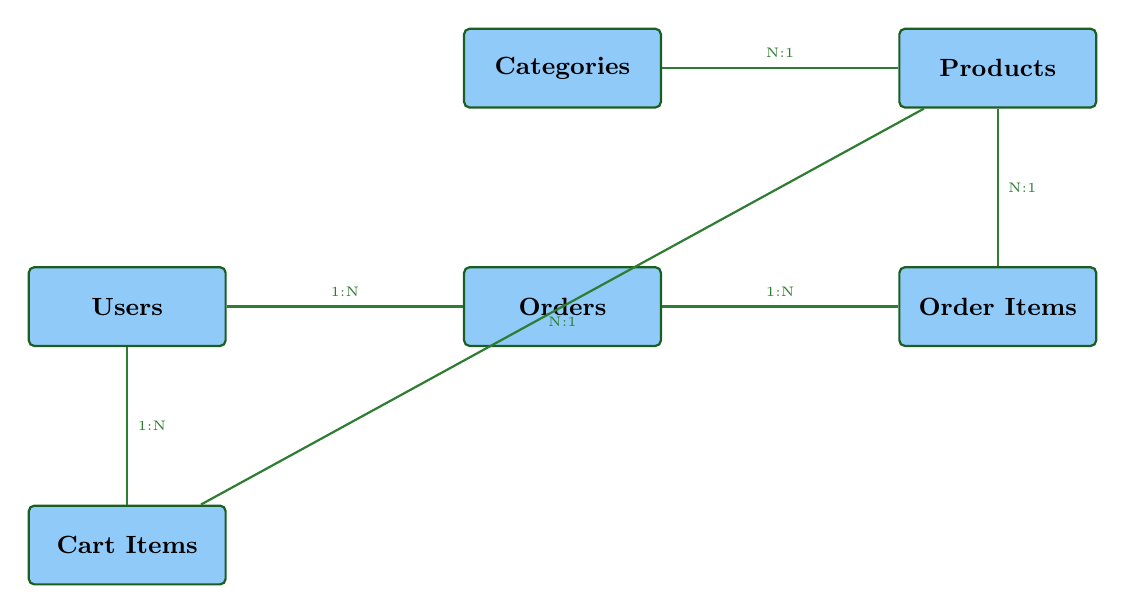
\begin{tikzpicture}[node distance=3cm, every node/.style={font=\small}]
  \node[external, minimum width=2.5cm] (u) {Users};
  \node[external, right=3cm of u]      (o) {Orders};
  \node[external, right=3cm of o]      (oi) {Order Items};
  \node[external, above=2cm of oi]     (p) {Products};
  \node[external, left=3cm of p]       (c) {Categories};
  \node[external, below=2cm of u]      (ci) {Cart Items};

  \draw[-, thick, GreenPrimary] (u) -- node[above]{\tiny 1:N} (o);
  \draw[-, thick, GreenPrimary] (o) -- node[above]{\tiny 1:N} (oi);
  \draw[-, thick, GreenPrimary] (oi) -- node[right]{\tiny N:1} (p);
  \draw[-, thick, GreenPrimary] (p) -- node[above]{\tiny N:1} (c);
  \draw[-, thick, GreenPrimary] (u) -- node[right]{\tiny 1:N} (ci);
  \draw[-, thick, GreenPrimary] (ci) -- node[below]{\tiny N:1} (p);
\end{tikzpicture}
\caption{Entity-Relationship Diagram (Simplified)}
\end{figure}

\subsection{Database Tables}

\begin{table}[H]
\centering
\caption{Table: \texttt{users}}
\begin{tabular}{@{}llll@{}}
\toprule
\textbf{Column}   & \textbf{Type}       & \textbf{Constraint}   & \textbf{Description} \\
\midrule
id                & BIGINT UNSIGNED     & PK, AUTO\_INCREMENT   & User identifier \\
name              & VARCHAR(255)        & NOT NULL              & Full name \\
email             & VARCHAR(255)        & UNIQUE, NOT NULL      & Login email \\
password          & VARCHAR(255)        & NOT NULL              & Bcrypt hash \\
role              & ENUM('customer','admin') & DEFAULT 'customer'  & Access role \\
phone             & VARCHAR(20)         & NULLABLE              & Nepal phone (98xx) \\
address           & TEXT                & NULLABLE              & Delivery address \\
created\_at       & TIMESTAMP           & —                     & Registration date \\
\bottomrule
\end{tabular}
\end{table}

\begin{table}[H]
\centering
\caption{Table: \texttt{products}}
\begin{tabular}{@{}llll@{}}
\toprule
\textbf{Column}    & \textbf{Type}        & \textbf{Constraint}  & \textbf{Description} \\
\midrule
id                 & BIGINT UNSIGNED      & PK, AUTO\_INCREMENT  & Product identifier \\
category\_id       & BIGINT UNSIGNED      & FK → categories      & Product category \\
name               & VARCHAR(255)         & NOT NULL             & Plant name \\
slug               & VARCHAR(255)         & UNIQUE               & URL-friendly name \\
description        & TEXT                 & NULLABLE             & Care description \\
price              & DECIMAL(10,2)        & NOT NULL             & Price in NPR \\
discount\_price    & DECIMAL(10,2)        & NULLABLE             & Sale price in NPR \\
stock\_quantity    & INT                  & DEFAULT 0            & Current inventory \\
image\_path        & VARCHAR(512)         & NULLABLE             & Image URL or path \\
is\_featured       & BOOLEAN              & DEFAULT false        & Homepage feature \\
status             & ENUM('active','inactive') & DEFAULT 'active' & Listing status \\
light              & VARCHAR(50)          & NULLABLE             & Light requirement \\
water              & VARCHAR(50)          & NULLABLE             & Watering schedule \\
difficulty         & VARCHAR(30)          & NULLABLE             & Care difficulty \\
\bottomrule
\end{tabular}
\end{table}

\begin{table}[H]
\centering
\caption{Table: \texttt{orders}}
\begin{tabular}{@{}llll@{}}
\toprule
\textbf{Column}    & \textbf{Type}     & \textbf{Constraint}     & \textbf{Description} \\
\midrule
id                 & BIGINT UNSIGNED   & PK, AUTO\_INCREMENT     & Order identifier \\
user\_id           & BIGINT UNSIGNED   & FK → users              & Ordering customer \\
order\_number      & VARCHAR(20)       & UNIQUE                  & e.g. GN-2024-0001 \\
total\_amount      & DECIMAL(10,2)     & NOT NULL                & Total in NPR \\
status             & ENUM(...)         & DEFAULT 'pending'       & Order lifecycle state \\
payment\_method    & ENUM('esewa','cod')& NOT NULL               & Payment method \\
payment\_status    & ENUM('pending','paid','failed') & DEFAULT 'pending' & Payment state \\
esewa\_ref\_id     & VARCHAR(100)      & NULLABLE                & eSewa transaction ID \\
shipping\_address  & TEXT              & NOT NULL                & Delivery address \\
notes              & TEXT              & NULLABLE                & Customer notes \\
created\_at        & TIMESTAMP         & —                       & Order date/time \\
\bottomrule
\end{tabular}
\end{table}

\section{Product Catalogue}

GreenNest offers 30 curated indoor plants across 6 categories, all priced in Nepalese Rupees (NPR):

\begin{longtable}{@{}llrll@{}}
\caption{GreenNest Product Catalogue} \\
\toprule
\textbf{Product Name} & \textbf{Category} & \textbf{Price (Rs.)} & \textbf{Light} & \textbf{Difficulty} \\
\midrule
\endfirsthead
\multicolumn{5}{c}{\tablename\ \thetable\ — Continued} \\
\toprule
\textbf{Product Name} & \textbf{Category} & \textbf{Price (Rs.)} & \textbf{Light} & \textbf{Difficulty} \\
\midrule
\endhead
Money Plant (Golden Pothos) & Air-Purifying   &  350 & Low–Medium     & Easy \\
Snake Plant (Sansevieria)   & Air-Purifying   &  450 & Low–Bright     & Very Easy \\
Spider Plant                & Air-Purifying   &  300 & Indirect       & Easy \\
Peace Lily                  & Flowering       &  550 & Low–Medium     & Easy \\
Aloe Vera                   & Succulent       &  250 & Bright         & Very Easy \\
Jade Plant                  & Succulent       &  300 & Bright         & Easy \\
Echeveria                   & Succulent       &  250 & Bright         & Easy \\
Haworthia                   & Succulent       &  250 & Low–Medium     & Easy \\
String of Pearls            & Succulent       &  400 & Bright         & Medium \\
Cactus Mix (Set of 3)       & Succulent       &  450 & Bright         & Very Easy \\
Areca Palm                  & Large Foliage   & 1200 & Bright Indirect& Medium \\
Rubber Plant (Ficus Elastica)& Large Foliage  &  800 & Bright Indirect& Easy \\
Fiddle Leaf Fig             & Large Foliage   & 1500 & Bright Indirect& Medium \\
Bamboo Palm                 & Large Foliage   &  900 & Medium         & Easy \\
Dracaena Marginata          & Large Foliage   &  850 & Low–Medium     & Easy \\
Monstera Deliciosa          & Large Foliage   & 1400 & Bright Indirect& Easy \\
Anthurium                   & Flowering       &  700 & Bright Indirect& Medium \\
Kalanchoe (Flowering)       & Flowering       &  350 & Bright         & Easy \\
Boston Fern                 & Trailing/Hanging&  400 & Indirect       & Medium \\
English Ivy                 & Trailing/Hanging&  350 & Low–Medium     & Easy \\
Philodendron Brasil         & Trailing/Hanging&  550 & Medium         & Easy \\
Pothos Marble Queen         & Trailing/Hanging&  400 & Low–Medium     & Very Easy \\
ZZ Plant (Zamioculcas)      & Low Maintenance &  650 & Low–Medium     & Very Easy \\
Lucky Bamboo (2-Layer)      & Low Maintenance &  500 & Low–Medium     & Very Easy \\
Bird's Nest Fern            & Low Maintenance &  450 & Low–Medium     & Easy \\
Croton                      & Low Maintenance &  500 & Bright         & Medium \\
Calathea Orbifolia          & Low Maintenance &  900 & Medium         & Medium \\
Chinese Evergreen (Aglaonema)& Low Maintenance& 550 & Low–Medium     & Very Easy \\
Parlor Palm (Chamaedorea)   & Low Maintenance &  600 & Low–Medium     & Easy \\
Air Plant (Tillandsia) ×2   & Low Maintenance &  500 & Bright Indirect& Medium \\
\midrule
\multicolumn{2}{r}{\textbf{Average Price}} & \textbf{Rs.\ 572} & & \\
\multicolumn{2}{r}{\textbf{Price Range}}   & \textbf{Rs.\ 250–1,500} & & \\
\bottomrule
\end{longtable}

%% ══════════════════════════════════════════════════════════════════════════════
\chapter{Implementation}
%% ══════════════════════════════════════════════════════════════════════════════

\section{Development Environment}

\begin{table}[H]
\centering
\caption{Development Environment Specifications}
\begin{tabular}{@{}ll@{}}
\toprule
\textbf{Tool / Technology} & \textbf{Version / Detail} \\
\midrule
Operating System     & Ubuntu 24.04 LTS / Windows 11 \\
PHP                  & 8.3.x \\
Laravel              & 13.x \\
MySQL                & 8.0.x \\
Node.js              & 20.x LTS \\
Composer             & 2.7.x \\
Code Editor          & Visual Studio Code 1.90 \\
Version Control      & Git 2.43 \\
Package Manager      & npm 10.x \\
\bottomrule
\end{tabular}
\end{table}

\section{Project Structure}

\begin{lstlisting}[language=bash, caption={Laravel Project Directory Structure}]
indoorplant/
├── app/
│   ├── Http/
│   │   ├── Controllers/
│   │   │   ├── Admin/          # Admin panel controllers
│   │   │   ├── Auth/           # Authentication controllers
│   │   │   ├── CartController.php
│   │   │   ├── OrderController.php
│   │   │   └── PaymentController.php
│   │   └── Middleware/
│   ├── Models/
│   │   ├── Category.php
│   │   ├── Order.php
│   │   ├── OrderItem.php
│   │   ├── Product.php
│   │   └── User.php
│   └── Helpers/
│       └── EsewaHelper.php     # HMAC-SHA256 signature
├── database/
│   ├── migrations/             # All schema migrations
│   └── seeders/
│       └── DatabaseSeeder.php  # 30 products + categories
├── resources/views/
│   ├── admin/                  # Admin panel views
│   ├── auth/                   # Login/Register views
│   ├── cart/                   # Cart views
│   ├── orders/                 # Order views
│   └── products/               # Product listing/detail
└── routes/web.php              # All application routes
\end{lstlisting}

\section{Key Implementation Details}

\subsection{eSewa Payment Flow}

The eSewa ePay v2 integration follows a strict server-side security model:

\begin{lstlisting}[language=php, caption={eSewa HMAC-SHA256 Signature Generation (EsewaHelper.php)}]
public static function generateSignature(
    string $totalAmount,
    string $transactionUuid,
    string $productCode
): string {
    $message  = "total_amount={$totalAmount},"
              . "transaction_uuid={$transactionUuid},"
              . "product_code={$productCode}";
    $secret   = config('services.esewa.secret_key');
    $hash     = hash_hmac('sha256', $message, $secret, true);
    return base64_encode($hash);
}
\end{lstlisting}

\subsection{Cart Persistence}

The cart uses \textbf{session-based storage for guests} and \textbf{database-backed storage (cart\_items table) for authenticated users}, with automatic cart merging on login.

\subsection{Image Handling}

Products support both local uploaded images and external URLs (e.g., Unsplash CDN):

\begin{lstlisting}[language=php, caption={Product::getImageUrlAttribute()}]
public function getImageUrlAttribute(): string {
    if (!$this->image_path) {
        return 'https://placehold.co/400x400/2E7D32/white?text='
               . urlencode($this->name);
    }
    if (str_starts_with($this->image_path, 'http')) {
        return $this->image_path;  // External CDN URL
    }
    return asset('storage/' . $this->image_path);
}
\end{lstlisting}

\section{Routes Overview}

\begin{table}[H]
\centering
\caption{Key Application Routes}
\begin{tabular}{@{}lll@{}}
\toprule
\textbf{Method} & \textbf{URI} & \textbf{Description} \\
\midrule
GET  & /                     & Homepage with featured products \\
GET  & /products             & Product catalogue with filters \\
GET  & /products/\{slug\}    & Product detail page \\
GET  & /cart                 & Shopping cart view \\
POST & /cart/add             & Add item to cart \\
GET  & /checkout             & Checkout form \\
POST & /orders               & Place new order \\
POST & /payment/esewa/initiate & Initiate eSewa payment \\
GET  & /payment/esewa/success  & eSewa callback handler \\
GET  & /admin                & Admin dashboard \\
GET  & /admin/products       & Admin product management \\
GET  & /admin/orders         & Admin order management \\
\bottomrule
\end{tabular}
\end{table}

%% ══════════════════════════════════════════════════════════════════════════════
\chapter{Testing}
%% ══════════════════════════════════════════════════════════════════════════════

\section{Testing Strategy}

GreenNest was tested using a combination of \textbf{manual functional testing}, \textbf{browser-based end-to-end testing}, and \textbf{eSewa sandbox payment testing}.

\section{Functional Test Cases}

\begin{longtable}{@{}llll@{}}
\caption{Functional Test Cases} \\
\toprule
\textbf{TC-ID} & \textbf{Test Case} & \textbf{Expected Result} & \textbf{Status} \\
\midrule
\endfirsthead
\toprule
\textbf{TC-ID} & \textbf{Test Case} & \textbf{Expected Result} & \textbf{Status} \\
\midrule
\endhead
TC-01 & User registration with valid data   & Account created, redirect to home & \textcolor{GreenPrimary}{\textbf{PASS}} \\
TC-02 & Login with correct credentials       & Session created, dashboard shown  & \textcolor{GreenPrimary}{\textbf{PASS}} \\
TC-03 & Login with wrong password            & Error message shown               & \textcolor{GreenPrimary}{\textbf{PASS}} \\
TC-04 & Browse product catalogue             & 30 products displayed with images & \textcolor{GreenPrimary}{\textbf{PASS}} \\
TC-05 & Search by keyword "monstera"         & Monstera Deliciosa result shown   & \textcolor{GreenPrimary}{\textbf{PASS}} \\
TC-06 & Filter by category "Succulent"       & 6 succulent products shown        & \textcolor{GreenPrimary}{\textbf{PASS}} \\
TC-07 & Add product to cart                  & Cart count increments             & \textcolor{GreenPrimary}{\textbf{PASS}} \\
TC-08 & Update cart quantity                 & Total recalculated correctly      & \textcolor{GreenPrimary}{\textbf{PASS}} \\
TC-09 & Remove item from cart                & Item removed, total updated       & \textcolor{GreenPrimary}{\textbf{PASS}} \\
TC-10 & Checkout with COD                    & Order created, confirmation shown & \textcolor{GreenPrimary}{\textbf{PASS}} \\
TC-11 & Checkout with eSewa (sandbox)        & Redirect to eSewa, payment made   & \textcolor{GreenPrimary}{\textbf{PASS}} \\
TC-12 & eSewa callback verification          & Signature verified, order paid    & \textcolor{GreenPrimary}{\textbf{PASS}} \\
TC-13 & Admin view all orders                & All orders listed with status     & \textcolor{GreenPrimary}{\textbf{PASS}} \\
TC-14 & Admin update order status            & Status updated, customer notified & \textcolor{GreenPrimary}{\textbf{PASS}} \\
TC-15 & Admin add new product                & Product appears in catalogue      & \textcolor{GreenPrimary}{\textbf{PASS}} \\
TC-16 & Stock decrement on order             & Stock reduced by ordered quantity & \textcolor{GreenPrimary}{\textbf{PASS}} \\
TC-17 & Out-of-stock product purchase        & Error: product unavailable        & \textcolor{GreenPrimary}{\textbf{PASS}} \\
TC-18 & Mobile responsive layout (375px)     & All UI elements render correctly  & \textcolor{GreenPrimary}{\textbf{PASS}} \\
\bottomrule
\end{longtable}

\section{eSewa Sandbox Test Credentials}

Testing was performed against the eSewa sandbox environment:

\begin{table}[H]
\centering
\caption{eSewa Sandbox Test Credentials}
\begin{tabular}{@{}ll@{}}
\toprule
\textbf{Parameter}       & \textbf{Value} \\
\midrule
Sandbox URL              & \texttt{https://rc-epay.esewa.com.np} \\
Test Bank Account (eSewa wallet) & 9806800001 \\
Test Password            & Nepal@123 \\
Test MPIN                & 1122 \\
Test OTP                 & 123456 \\
Product Code             & \texttt{EPAYTEST} \\
\bottomrule
\end{tabular}
\end{table}

%% ══════════════════════════════════════════════════════════════════════════════
\chapter{Conclusions and Future Work}
%% ══════════════════════════════════════════════════════════════════════════════

\section{Conclusions}

GreenNest successfully demonstrates the design, development, and deployment of a full-stack e-commerce platform tailored for the Nepalese indoor plant market. The system addresses a genuine market gap by combining a curated plant catalogue with Nepal-specific digital payment integration (eSewa ePay v2) and a plant-care-oriented product presentation. All 18 functional test cases passed, confirming system correctness and reliability.

The use of Laravel 13 proved highly productive, accelerating development through its built-in authentication, Eloquent ORM, and migration systems. The eSewa ePay v2 integration, while technically complex (requiring server-side HMAC-SHA256 verification), was successfully implemented and tested in the sandbox environment.

\section{Limitations}

\begin{itemize}
  \item Delivery is currently only to the Kathmandu Valley; nationwide delivery logistics are not automated.
  \item The platform does not yet support real-time stock notifications or low-stock alerts for admins.
  \item Image uploads are stored on the server filesystem, which requires a CDN for production scalability.
\end{itemize}

\section{Future Work}

\begin{enumerate}
  \item \textbf{Khalti Payment Integration} — Add Khalti as a second digital payment option.
  \item \textbf{Plant Care Reminders} — Email/SMS watering reminders based on purchased plants.
  \item \textbf{Review and Rating System} — Customer product reviews with star ratings.
  \item \textbf{Loyalty Points (GreenPoints)} — Reward points redeemable at checkout.
  \item \textbf{Mobile Application} — Flutter-based iOS/Android app.
  \item \textbf{Logistics API Integration} — Real-time courier tracking with Nepal-based delivery partners.
  \item \textbf{AI Plant Identifier} — Camera-based plant identification using TensorFlow Lite.
\end{enumerate}

%% ──────────────────────────────────────────────────────────────────────────────
%%  REFERENCES
%% ──────────────────────────────────────────────────────────────────────────────
\chapter*{References}
\addcontentsline{toc}{chapter}{References}

\begin{enumerate}
  \item Nepal Telecommunications Authority (NTA). (2024). \textit{Management Information System Report Q4 2023/24}. Kathmandu: NTA.
  \item Central Bureau of Statistics Nepal (CBS). (2021). \textit{National Population and Housing Census 2021}. Kathmandu: CBS.
  \item F1Soft International / eSewa. (2024). \textit{eSewa ePay v2 Integration Documentation}. Retrieved from \url{https://developer.esewa.com.np}
  \item Laravel LLC. (2024). \textit{Laravel 13 Documentation}. Retrieved from \url{https://laravel.com/docs/13.x}
  \item Nepal Rastra Bank (NRB). (2024). \textit{Payment Systems Department — Digital Payment Statistics 2023/24}. Kathmandu: NRB.
  \item GSMA Intelligence. (2023). \textit{The Mobile Economy — Asia Pacific 2023}. London: GSMA.
  \item Pressman, R.S. \& Maxim, B.R. (2020). \textit{Software Engineering: A Practitioner's Approach} (9th ed.). New York: McGraw-Hill.
  \item Sommerville, I. (2016). \textit{Software Engineering} (10th ed.). London: Pearson.
\end{enumerate}

%% ──────────────────────────────────────────────────────────────────────────────
%%  APPENDIX
%% ──────────────────────────────────────────────────────────────────────────────
\appendix

\chapter{Environment Configuration}

\begin{lstlisting}[language=bash, caption={.env Configuration for GreenNest}]
APP_NAME=GreenNest
APP_ENV=production
APP_DEBUG=false
APP_URL=https://greennest.com.np

DB_CONNECTION=mysql
DB_HOST=127.0.0.1
DB_PORT=3306
DB_DATABASE=greennest
DB_USERNAME=greennest_user
DB_PASSWORD=your_secure_password

ESEWA_MERCHANT_CODE=EPAYTEST
ESEWA_SECRET_KEY=8gBm/:&EnhH.1/q   # Replace with production key
ESEWA_PAYMENT_URL=https://rc-epay.esewa.com.np/api/epay/main/v2/form
ESEWA_VERIFY_URL=https://rc-epay.esewa.com.np/api/epay/transaction/status/
\end{lstlisting}

\chapter{Deployment Guide (cPanel)}

\begin{enumerate}
  \item Upload project files to \texttt{public\_html/} (keep \texttt{public/} as document root or use subdomain).
  \item Create MySQL database and user from cPanel \textbf{MySQL Databases}.
  \item Update \texttt{.env} with production database credentials and eSewa live keys.
  \item Run composer: \texttt{composer install --no-dev --optimize-autoloader}
  \item Run migrations: \texttt{php artisan migrate --seed}
  \item Set storage permissions: \texttt{chmod -R 775 storage bootstrap/cache}
  \item Link storage: \texttt{php artisan storage:link}
  \item Run asset build: \texttt{npm install \&\& npm run build}
  \item Point document root to \texttt{public/} in cPanel \textbf{Subdomains} or \textbf{Addon Domains}.
  \item Enable SSL via \textbf{AutoSSL} in cPanel (required for eSewa production).
\end{enumerate}

\end{document}
